\documentclass[]{article}
\usepackage[T1]{fontenc}
\usepackage[utf8]{inputenc}
\usepackage[swedish]{babel}
\usepackage[margin=1.7in]{geometry}
\usepackage{mathtools}
\usepackage{graphicx}
\usepackage{listings}



%opening
\title{Laboration II - Modellprovning för CTL \\ DD1351 Logik för dataloger }
\author{Emil Ståhl}

\begin{document}

\setlength\parindent{0pt}
\maketitle

\section{Introduktion}
Denna rapport behandlar implementering och testning av ett kontrollprogram för temporallogik och modellbaserad systemutveckling skrivet i prolog. Indata till programmet är en fil med modellen, sanningstilldelningslistan, starttillståndet samt formeln. Programmet returnerar antingen \texttt{"yes"} eller \texttt{"no"} beroende på om modellen med dess tillstånd och övergångar är korrekt eller ej. Programmet har stöd för samtliga temporala kvantifierare för att uttrycka sanning över sekvenser av valueringar, en komplett lista över dessa återfinns i appendix. 

\section{Generell beskrivning av algoritmen}
Algoritmen startar i predikatet \texttt{check} med värdena från indata tillsammans med en tom lista som håller reda på vilka tillstånd som har besökts. Syftet med \texttt{check} är att verifiera varje delformel rekursivt. För att göra detta använder \texttt{check} sig av två andra predikat, \texttt{check\_all} och \texttt{check\_exist}, som rekursivt kontrollerar A-formler respektive E-formler. För att upptäcka slingor i modellen skapas en lista  \texttt{visited} som bevarar alla tillstånd som redan undersöks. Varje predikat check börjar därav med att kontrollera om tillståndet  \texttt{S} finns i listan  \texttt{visited}. Om \texttt{S} inte finns i listan så utförs resten av predikatet.

\section{Modellering}
Den modell som konstruerats visualiseras med en tillståndsgraf i figur 1. Modellen beskriver en uttagsautomat där en användare initialt möts av en startskärm där en pinkod ska matas in. Om pinkoden är korrekt kan ett valfritt saldo väljas. Om pinkoden är felaktig återgår proceduren till startskärmen. Om det saldo som matats in av användaren är godkänt slutförs uttaget och proceduren avslutas genom att återgå till startskärmen. Användaren kan i alla tillstånd avbryta proceduren.




\subsection{Möjliga tillstånd för modellen}
Modellen består av fem olika tillstånd samt fyra atomer och beskrivs visuellt i figur 1. 
\begin{figure}[h]
\centering
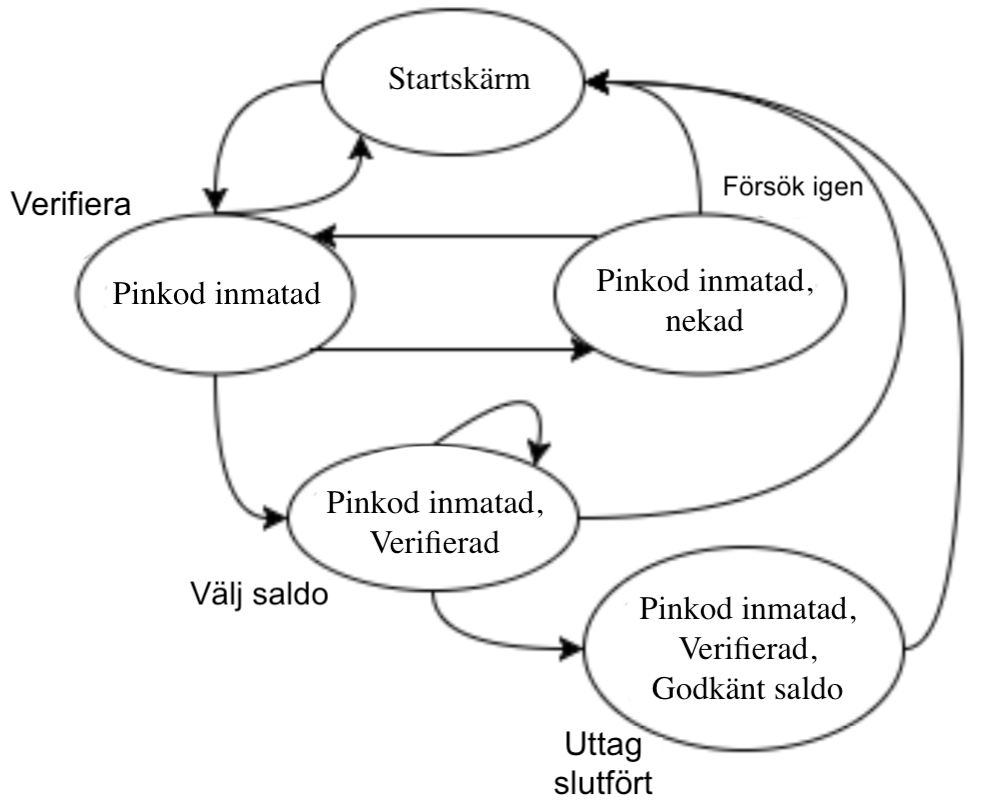
\includegraphics[width=0.7\textwidth]{modell.png}
\caption{Tillståndsgraf}
\end{figure}

Dessa tillstånd och atomer består av:\\

Tillstånd:
\begin{itemize}
  \item Startskärm
  \item Verifiera
  \item Försök igen
  \item Välj saldo
  \item Uttag slutfört
\end{itemize}

Atomer:
\begin{itemize}
  \item Pinkod inmatad
  \item Nekad
  \item Verifiera
  \item Godkänt saldo
\end{itemize}

\clearpage

\subsection{Representation av modell i prolog}

\begin{verbatim}

% Tillstånden är: s(startskärm), v(verifiera), fi(försök igen), vs(välj saldo) och 
% us(uttag slutfört).

[
  [s, [v]],
  [v, [s, v, fi, vs]], 
  [fi, [s, v]],
  [vs, [s, vs, us] ],
  [us, [s] ]
].

[
  [s, [ ] ],
  [v, [pi]],
  [fi [pi, n]],
  [vs, [pi, v]],
  [us, [pi,  v,  gs]]
].

s.

ef(and(and(pi,v),gs)).

\end{verbatim}

\section{CTL-Formler}
Nedan specificeras två systemegenskaper uttryckta som CTL-formler relaterade till modellen som beskrivits ovan. Den första är hållbar medan den senare är ohållbar. 

\subsection{Hållbar systemegenskap}

I denna specificerade systemegenskap existerar det en väg där det sedermera är möjligt att ta ut pengar:\\

\texttt{ef(and(and(pi,v),gs))}.



\subsection{Ohållbar systemegenskap}

I denna specificerade systemegenskap existerar det en väg där något av de efterföljande stegen inte är startskärmen:\\

\texttt{ef(not(ex(not(pi))))}

\section{Verifiering av systemegenskaper}

Med den implementerade modellprovaren verifierades de definierade systemegenskaperna beskrivna i avsnitt 4. Resultatet blev som förväntat att modellprovaren bedömde den hållbara systemegenskapen som sann och den ohållbara som falsk. Vilket var det resultat som förväntades.\\

Mer specifikt så returnerar modellprovaren sant för den hållbara systemegenskapen eftersom det existerar en väg där vardera tillstånd pi, v, gs kommer att vara sanna, dvs i s. Liknande gäller för den ohållbara systemegenskapen där alla tillstånd kan övergå till s då pi är invalid, vilket medför att modellprovaren returnerar falskt. 
\\\\
Angående de fördefinierade testfallen returnerades korrekt resultat för samtliga 730 stycken testfiler. 

\clearpage
\section*{Appendix}
\appendix

\section{Predikat}

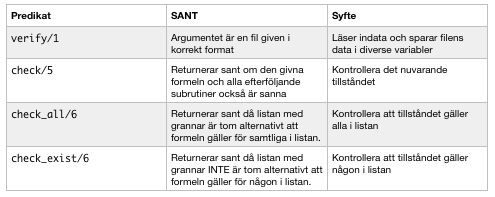
\includegraphics[width=0.99\textwidth]{Predikat.png}

\section{Temporala kvantifierare}
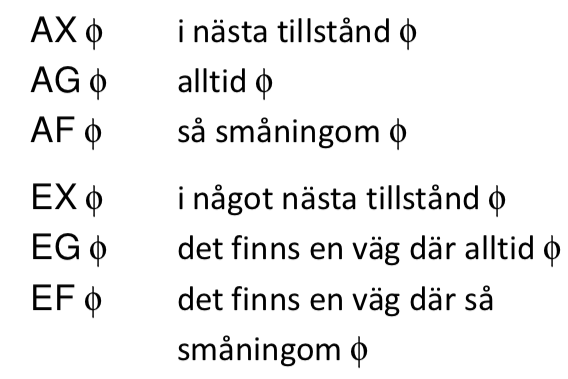
\includegraphics[width=0.6\textwidth]{semantik.png}

\section{Programkod}

\begin{verbatim}
	verify(Input) :-
	see(Input), read(T), read(L), read(S), read(F), seen,
	check(T, L, S, [], F).

check(_, L, S, [], X) :-
	member([S,Z],L), 
	member(X, Z).

check(_, L, S, [], neg(X)) :-
	member([S,Z],L), 
	\+ member(X, Z).

check(T, L, S, [], and(F,G)) :-
	check(T, L, S, [], F),
	check(T, L, S, [], G).

check(T, L, S, [], or(F,G)) :- 
	check(T, L, S, [], F);
	check(T, L, S, [], G).

check(T, L, S, [], ax(F)) :-
	member([S, Z], T), 
	check_all(T, L, Z, [], F, F). 

check(T, L, S, visited, ag(F)):-
	member(S, visited).
check(T, L, S, visited, ag(F)) :-
	\+ member(S, visited),
	check(T, L, S, [], F), 
	member([S, Z], T), 
	check_all(T, L, Z, [S|visited], F, ag(F)). 

check(T, L, S, visited, af(F)):-
	\+ member(S, visited),
	check(T, L, S, [], F).

check(T, L, S, visited, af(F)) :- 
	\+ member(S, visited),
	member([S, Z], T), 
	check_all(T, L, Z, [S|visited], F, af(F)). 

check(T, L, S, visited, eg(F)):-
	member(S, visited).
check(T, L, S, visited, eg(F)) :-
	\+ member(S, visited),
	check(T, L, S, [], F),
	member([S, Z], T), 
	check_exist(T, L, Z, [S|visited], F, eg(F)). 

check(T, L, S, visited, ef(F)):-
	\+ member(S, visited),
	check(T, L, S, [], F). 
check(T, L, S, visited, ef(F)) :-
	\+ member(S, visited),
	member([S, Z], T), 
	check_exist(T, L, Z, [S|visited], F, ef(F)).

check(T, L, S, [], ex(F)) :-
	member([S, Z], T), 
	check_exist(T, L, Z, [], F, F).

check_all(_,_,[],_,_,_). 
check_all(T, L, [H|TAIL], visited, X, A) :-
	check(T, L, H, visited, A), 
	check_all(T, L, TAIL, visited, X, A). 

check_exist(_,_,[],_,_,_):- fail.
check_exist(T, L, [H|TAIL], visited, X, A) :-
	check(T, L, H, visited, A); 
	check_exist(T, L, TAIL, visited, X, A). 
	
\end{verbatim}

\end{document}